%% Template for ENG 401 reports
%% by Robin Turner
%% Adapted from the IEEE peer review template

\documentclass[journal,12pt,onecolumn,a4paper]{IEEEtran}
\usepackage{cite} % Tidies up citation numbers.
\usepackage{url} % Provides better formatting of URLs.
\usepackage[utf8]{inputenc} % Allows Turkish characters.
\usepackage{booktabs} % Allows the use of \toprule, \midrule and \bottomrule in tables for horizontal lines
\usepackage{graphicx}
\usepackage{amsmath}
\usepackage{float}
\usepackage{multicol}
\usepackage{listings}
\usepackage[justification=centering]{caption}
\usepackage[numbered,framed]{matlab-prettifier}
\usepackage[export]{adjustbox}
\usepackage{color} %red, green, blue, yellow, cyan, magenta, black, white
\definecolor{mygreen}{RGB}{28,172,0} % color values Red, Green, Blue
\definecolor{mylilas}{RGB}{170,55,241}

\graphicspath{ {./assets/pics} }

\hyphenation{op-tical net-works semi-conduc-tor} % Corrects some bad hyphenation 
\lstset{language=Matlab,%
	basicstyle=\ttfamily,
    breaklines=true,%
    morekeywords={matlab2tikz},
    keywordstyle=\color{blue},%
    morekeywords=[2]{1}, keywordstyle=[2]{\color{black}},
    identifierstyle=\color{black},%
    stringstyle=\color{mylilas},
    commentstyle=\color{mygreen},%
    showstringspaces=false,%without this there will be a symbol in the places where there is a space
    emph=[1]{for,end,break},emphstyle=[1]\color{red}, %some words to emphasise
    %emph=[2]{word1,word2}, emphstyle=[2]{style},    
}


\begin{document}
\begin{titlepage}
	% paper title
	% can use linebreaks \\ within to get better formatting as desired
	\title{Interpolasi Numerik: Path Calculator}


	% author names and affiliations

	\author{Adrian Ardizza - 2006524896\\
		Alya Azhar Agharid - 2006462720\\
		Muhammad Athallah - 2006527481\\
		Stefanus Ndaru Wedhatama - 2006526812
	}

	% make the title area
	\maketitle
	\begin{abstract}
		The abstract does not only mention the paper but is the original paper shrunken to approximately 200 words. It states the purpose, reports the information obtained, and gives conclusions, and recommendations. In short, it summarizes the main points of the study adequately and accurately. It provides information from every major section in the body of the report in a dense and compact way. Past tense and active voice is appropriate when describing what was done. If there is any, it includes key statistical detail.

		Depending on the format you use, the abstract may come on the title page or at the beginning of the main report.

	\end{abstract}
	\tableofcontents
	\listoffigures
	\listoftables
\end{titlepage}

\IEEEpeerreviewmaketitle

\section{Pendahuluan}
Interpolasi merupakan teknik yang digunakan untuk membangun suatu fungsi yang melewati sebuah himpunan titik-titik diskret yang diketahui. Fungsi interpolasi memiliki aplikasi yang luas pada ilmu komputer karena dapat digunakan untuk menggambarkan berbagai kurva kompleks dengan \emph{computational cost} yang relatif murah apabila dibandingkan dengan metode \emph{brute force} (mencari seluruh titik yang memenuhi suatu kurva secara \emph{exhaustive}). Interpolasi beberapa titik diskret dapat dicapai dengan berbagai metode interpolasi seperti interpolasi konstan, interpolasi linear, interpolasi polinomial, dan interpolasi \emph{spline} yang menjadi topik dari paper ini.

Secara matematis, sebuah fungsi interpolasi dapat dinyatakan sebagai suatu fungsi \(P(x)\) di mana \(x\) adalah sebuah titik yang ingin diinterpolasi. Hasil dari fungsi tersebut adalah sebuah \emph{value} yang merupakan aproksimasi dari nilai fungsi \(f(x)\) yang melewati seluruh titik-titik diskret yang nilainya sudah diketahui.

Pada \emph{paper} ini, kami ingin mengeksplorasi pemanfaatan sebuah fungsi \emph{cubic spline}—atau lebih tepatnya fungsi \emph{cubic spline} dengan kondisi \emph{natural}—untuk melakukan \emph{smoothing} pada perubahan posisi suatu titik di interval waktu \([0, n]\). Cubic spline dapat didefinisikan sebagai suatu \emph{piecewise polynomial function} yang menginterpolasi sebuah himpunan titik dengan menggunakan sebuah \emph{cubic polynomial} sebagai fungsi dasarnya pada setiap interval.

Untuk sebuah input yang berisi \(n\) titik, akan terdapat \(n-1\) \emph{cubic function} yang menginterpolasi titik-titik tersebut di setiap interval. Pembangunan spline ini sendiri akan dijelaskan secara lebih mendetil pada bagian selanjutnya. Fungsi \emph{natural cubic spline} ini kemudian akan digunakan sebagai basis untuk suatu fungsi parametrik \((x(t), y(t))\) yang mengambil suatu \emph{array} berisi \emph{time-step} dengan resolusi \(r\) dan menginterpolasi (x, y) untuk input tersebut.

Output yang diharapkan dari fungsi tersebut adalah sebuah kurva parametrik menginterpolasi gerak titik seperti pada dua contoh berikut ini:

\begin{multicols}{2}
	\begin{figure}[H]
		\centering
		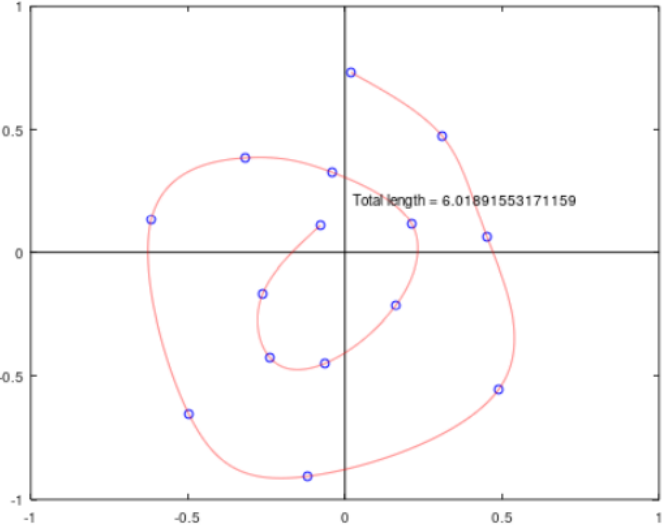
\includegraphics[max size={\textwidth/2}{\textheight}]{soal1-tc1}
		\caption{Contoh Graf Interpolasi \#1}
		\label{fig_tc1}
	\end{figure}
	\columnbreak
	\begin{figure}[H]
		\centering
		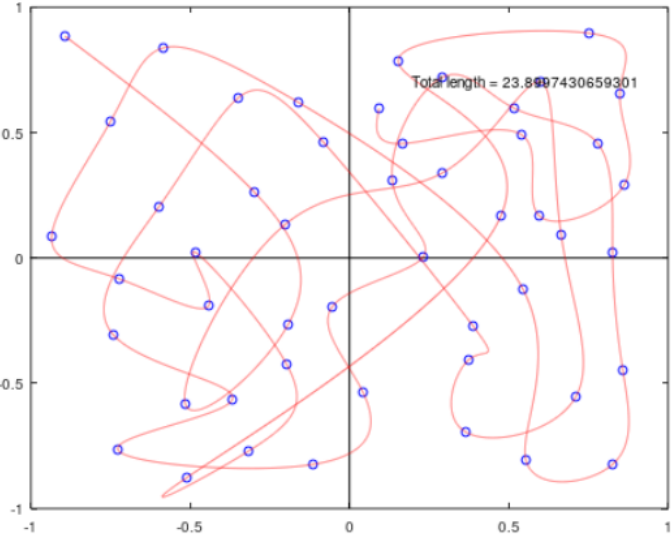
\includegraphics[max size={\textwidth/2}{\textheight}]{soal1-tc2}
		\caption{Contoh Graf Interpolasi \#2}
		\label{fig_sim2}
	\end{figure}
\end{multicols}

\pagebreak

\section{Membangun Fungsi (x(t), y(t))}
Pada bagian ini, kami akan membangun fungsi parametrik \((x(t), y(t))\) yang dapat menghasilkan output yang diharapkan dari tugas kali ini.

\subsection{Definisi Cubic Spline}
Apabila diberikan \(n + 1\) titik data \(x_i, y_i\), dimana \(a = x_0\) dan \(b = x_n\), maka fungsi \emph{cubic spline} \(S(x)\) adalah fungsi yang memenuhi syarat:
\begin{itemize}
	\item \(S(x) \in C^2[a, b]\)
	\item Pada setiap subinterval \([x_{i - 1}, x_i]\) dimana \(i = 1, ..., n\), \(S(x)\) adalah polinomial derajat 3.
	\item \(S(x_i) = y_i\) untuk semua \(i = 0, 1, ..., n\).
\end{itemize}

Sehingga kita dapat mendefinisikan fungsi \emph{cubic spline} \(S(x)\) sebagai:
\begin{equation}
	S(x) = \begin{cases}
		C_1(x) & x_0 \leq x \leq x_1  \\
		\dots                         \\
		C_i(x) & x_{i-1} < x \leq x_i \\
		\dots                         \\
		C_n(x) & x_{n-1} < x \leq x_n
	\end{cases}
\end{equation}
\begin{equation}
	\text{dimana }C_i = a_i + b_ix + c_ix^2 + d_ix^3
\end{equation}

Pada umumnya, sebuah \emph{cubic spline} harus memenuhi beberapa syarat:
\begin{itemize}
	\item Menginterpolasi titik-titik data: \(s_i(x_i) = y_i\)
	\item \(S(x)\) kontinu pada interval \([0, n]\): \(s_i{x_i+1} = y_{i + 1}\)
	\item Turunan pertama \(S(x)\) kontinu pada interval \([0, n]\): \(S_i'(x_{i + 1}) = s_{i + 1}'(x_{i + 1})\)
	\item Turunan kedua \(S(x)\) kontinu pada interval \([0, n]\): \(S_i''(x_{i + 1}) = S_{i + 1}''(x_{i + 1})\)
\end{itemize}

Selain itu, sebuah fungsi \emph{cubic spline} juga harus memenuhi sebuah \emph{boundary condition} untuk membentuk suatu sistem persamaan yang dapat diselesaikan. Pada tugas kali ini, \emph{boundary condition} yang digunakan adalah kondisi \emph{natural} yang didefinisikan sebagai:
\begin{equation}
	S_0''(x_0) = 0
\end{equation}
\begin{equation}
	S_{n-1}''(x_n) = 0
\end{equation}

Dari syarat-syarat tersebut, akan diperoleh suatu sistem persamaan linear yang dapat digunakan untuk mencari koefisien dari setiap \emph{piecewise cubic function} yang menginterpolasi interval \([a, b]\).

Setelah mendefinisikan syarat-syarat yang harus dipenuhi oleh \emph{cubic spline}, maka kita dapat mulai membangun definisi umum \emph{natural cubic spline} yang dapat diimplementasikan dengan menggunakan MATLAB. Terdapat dua pendekatan yang dapat dilakukan untuk membangun sistem ini, yakni secara \emph{top-down} ataupun secara \emph{bottom-up}.

Pendekatan \emph{top-down} dilakukan dengan mencari nilai-nilai koefisien \(a, b, c, d\) yang dapat memenuhi persamaan \(S_i(x) = a_i + b_ix + c_ix^2 + d_ix^3\). Pendekatan ini akan menghasilkan suatu sistem persamaan yang memiliki \(4n\) \emph{unknowns} dan \(4n\) \emph{equations}, dimana \(n\) adalah jumlah titik yang ingin diinterpolasi.

Sementara itu pendekatan \emph{bottom-up} dilakukan dengan pertama mendefinisikan sebuah fungsi \(S''(x)\) linear yang kemudian diintegrasikan untuk mendapatkan suatu fungsi \(S(x)\) kubik. Lalu kita dapat menggunakan syarat-syarat yang sudah didefinisikan pada bagian sebelumnya untuk mencari \emph{unknown terms} yang dihasilkan oleh proses integrasi dan mendefinisikan sistem persamaan yang mencari semua \emph{knot} pada \emph{spline} dan fungsi \emph{spline} pada setiap interval.

\subsection{Membangun Algoritma Natural Cubic Spline}
Kami akan menggunakan pendekatan \emph{bottom-up} untuk membangun algoritma \emph{Natural Cubic Spline} yang akan digunakan pada fungsi \((x(t), y(t))\).

Asumsikan bahwa:
\begin{itemize}
	\item Terdapat suatu himpunan berisi \(n\) titik data \((x_i, y_i)\) dimana \(x_1 < x_2 < \dots < x_n\)
	\item \(f(x)\) adalah polinomial dengan derajat \(\leq 3\) pada setiap subinterval \([x_i, x_{i + 1}]\)
	\item \(f(x)\), \(f'(x)\), \(f''(x)\) adalah fungsi kontinu untuk interval \(a \leq x \leq b\) sehingga:
	      \begin{itemize}
		      \item \(f_{i-1,i}(x_i) = f_{i, i+1}(x_i)\)
		      \item \(f_{i-1,i}'(x_i) = f_{i, i+1}'(x_i)\)
		      \item \(f_{i-1,i}''(x_i) = f_{i, i+1}''(x_i)\ = k_i\)
	      \end{itemize}
	      Dimana \(k_i\) adalah nilai turunan kedua \(f(x)\) pada segmen ke-i
\end{itemize}

Dengan asumsi tersebut, kita dapat mulai membangun fungsi \emph{interpolant} \(f_{i, i+1}(x)\) dengan asumsi fungsi tersebut adalah sebuah fungsi kubik. Karena fungsi tersebut merupakan suatu fungsi derajat tiga, maka turunan keduanya pada suatu \(x\) merupakan sebuah fungsi linear.

Ingat bahwa sebuah fungsi linear yang menginterpolasi dua titik dapat dicari menggunakan basis Lagrange, sehingga kita dapat mendefinisikan \(S''(x)\) sebagai berikut.
\begin{equation}
	f''_{i, i+1}(x) = k_i\frac{x-x_{i + 1}}{x_i - x_{i + 1}} + k_{i+1}\frac{x - x_i}{x_{i + 1} - x_i}
\end{equation}

Selanjutnya, kita dapat melakukan integrasi pada fungsi tersebut untuk mendapatkan \(f_{i, i+1}'(x)\) dan \(f_{i, i+1}(x)\).
\begin{equation}
	\begin{split}
		f_{i, i+1}'(x) & = \int f_{i, i+1}''(x) dx\\
		& = \int (k_i\frac{x-x_{i + 1}}{x_i - x_{i + 1}} + k_{i+1}\frac{x - x_i}{x_{i + 1} - x_i})dx\\
		& = \frac{k_i(x-x_{i+1})^2}{2(x_i-x_{i+1})} + \frac{k_{i+1}(x-x_{i})^2}{2(x_{i+1}-x_{i})} + C
	\end{split}
\end{equation}
\begin{equation}
	\begin{split}
		f_{i, i+1}(x) & = \int f_{i, i+1}'(x) dx\\
		& = \int (\frac{k_i(x-x_{i+1})^2}{2(x_i-x_{i+1})} + \frac{k_{i+1}(x-x_{i})^2}{2(x_{i+1}-x_{i})} + C)dx\\
		& = \frac{k_i(x-x_i)^3}{6(x_i - x_{i+1})} + \frac{k_{i+1}(x - x_i)^3}{6(x_{i+1} - x_i)} + Cx + D
	\end{split}
\end{equation}

Setelah mendapatkan fungsi \(f(x)\) dan \(f'(x)\), kita harus selanjutnya mencari nilai dari suku C dan D agar dapat menggunakan fungsi tersebut sebagai interpolant.
\begin{equation}
	C = A - B\\
\end{equation}
\begin{equation}
	D = -Ax_{i+1} + Bx_i
\end{equation}

Sehingga kita akan mendapatkan,
\begin{equation}
	\begin{split}
		f_{i, i+1}(x) & = \frac{k_i(x-x_i)^3}{6(x_i - x_{i+1})} + \frac{k_{i+1}(x - x_i)^3}{6(x_{i+1} - x_i)} + (A-B)x - Ax_{i+1} + Bx_i\\
		& = \frac{k_i(x-x_i)^3}{6(x_i - x_{i+1})} + \frac{k_{i+1}(x - x_i)^3}{6(x_{i+1} - x_i)} + A(x-x_{i+1}) - B(x-x_i)
	\end{split}
\end{equation}

Selanjutnya kita dapat menggunakan syarat-syarat dari fungsi \(S(x)\) untuk menemukan A dan B yang dapat menyelesaikan rumus di atas.

\begin{itemize}
	\item
	      \(f_{i, i+1}(x_i) = y_i\)

	      Apabila kita melakukan substitusi syarat ini ke persamaan di atas, maka kita akan mendapatkan:
	      \begin{equation*}
		      y_i = \frac{k_i(x_i - x_{i+1})^3}{6(x_i - x_{i+1})} + A(x_i - x_{i+1})
	      \end{equation*}
	      \begin{equation*}
		      A(x_i - x_{i+1}) = y_i - \frac{k_i(x_i - x_{i+1})^3}{6(x_i - x_{i+1})}
	      \end{equation*}
	      \begin{equation}
		      A = \frac{y_i}{x_i - x_{i+1}} - \frac{k_i}{6}(x_i - x_{i+1})
	      \end{equation}

	\item
	      \(f_{i, i+1}(x_{i+1}) = y_{i+1}\)

	      Apabila kita melakukan substitusi syarat ini ke persamaan di atas, maka kita akan mendapatkan:
	      \begin{equation*}
		      y_{i+1} = B(x_{i+1} - x_i) - \frac{k_{i+1}(x_{i+1}-x_i)^3}{6(x_i - x_{i + 1})}
	      \end{equation*}
	      \begin{equation*}
		      \begin{split}
			      B(x_{i+1} - x_i) & = y_{i+1} + \frac{k_{i+1}(x_{i+1}-x_i)^3}{6(x_i - x_{i + 1})}\\
			      & = y_{i+1} - \frac{k_{i+1}(x_{i+1}-x_i)^3}{6(x_{i + 1} - x_i)}
		      \end{split}
	      \end{equation*}
	      \begin{equation}
		      B = \frac{y_{i+1}}{(x_i - x_{i+1})} - \frac{k_{i+1}}{6}(x_i - x_{i+1})
	      \end{equation}
\end{itemize}

Setelah mendapatkan \(A\) dan \(B\) kita dapat melakukan substitusi kembali suku-suku tersebut ke \(f_{i, i+1}(x)\) untuk mendapatkan:
\begin{equation}
	\begin{split}
		f_{i, i+1}(x) & = \frac{k_i}{6}[\frac{x-x_{i+1}^3}{x_i-x_{i+1}} - (x - x_{i+1})(x_i - x_{i+1})]\\
		& - \frac{k_{i+1}}{6}[\frac{(x-x_i)^3}{x_i - x_{i+1}} - (x-x_i)(x_i - x_{i+1})]\\
		& + \frac{y_i(x-x_{i+1}) - y_{i+1}(x-x_i)}{x_i - x_{i+1}}
	\end{split}
\end{equation}

Selanjutnya kita harus mencari vektor \(k\) yang dapat digunakan untuk menghitung nilai interpolasi. Ingat bahwa suatu fungsi \emph{spline} harus memenuhi:
\begin{equation*}
	f_{i-1, i}'(x_i) = f_{i, i+1}'(x_i)
\end{equation*}
Dimana \(i = 2, 3, \dots, n-1\) karena diketahui bahwa \(k_i = k_n = 0\) berdasarkan \emph{natural boundary condition}. Maka kita akan mendapatkan persamaan sebagai berikut.
\begin{equation*}
	\begin{split}
		f'_{i, i+1}(x_i) & = \frac{k_i}{6}[\frac{3(x-x_{i+1})^2}{x_i - x_{i+1}} - (x_i - x_{i+1})]\\
		& - \frac{k_{i+1}}{6}[\frac{3(x-x_i)^2}{x_i - x_{i+1}} - (x_i - x_{i+1})]\\
		& + \frac{y_i - y_{i+1}}{x_i - x_{i+1}}
	\end{split}
\end{equation*}

\begin{equation*}
	\begin{split}
		f'_{i-1, i}(x_i) & = \frac{k_{i-1}}{6}[\frac{3(x-x_{i})^2}{x_{i-1} - x_{i}} - (x_{i-1} - x_{i})]\\
		& - \frac{k_{i}}{6}[\frac{3(x-x_{i-1})^2}{x_{i-1} - x_{i}} - (x_{i-1} - x_{i})]\\
		& + \frac{y_{i-1} - y_{i}}{x_{i-1} - x_{i}}
	\end{split}
\end{equation*}

\begin{equation*}
	\frac{k_i}{6}[\frac{3(x-x_{i+1})^2}{x_i - x_{i+1}} - (x_i - x_{i+1})] - \frac{k_{i+1}}{6}[\frac{3(x-x_i)^2}{x_i - x_{i+1}} - (x_i - x_{i+1})] + \frac{y_i - y_{i+1}}{x_i - x_{i+1}}
\end{equation*}
\begin{equation*}
	=
\end{equation*}
\begin{equation*}
	\frac{k_{i-1}}{6}[\frac{3(x-x_{i})^2}{x_{i-1} - x_{i}} - (x_{i-1} - x_{i})] - \frac{k_{i}}{6}[\frac{3(x-x_{i-1})^2}{x_{i-1} - x_{i}} - (x_{i-1} - x_{i})] + \frac{y_{i-1} - y_{i}}{x_{i-1} - x_{i}}
\end{equation*}

Menyelesaikan persamaan tersebut akan menghasilkan sistem persamaan linear sebagai berikut.
\begin{equation}
	k_{i-1}(x_{i-1} - x_i) + 2k_i(x_{i-1} - x_{i+1}) + k_{i+1}(x_i - x_{i+1}) = 6(\frac{y_{i-1}-y_i}{x_{i-1}-x_i} - \frac{y_i-y_{i+1}}{x_i - x_{i+1}})
\end{equation}
Kita dapat juga menyatakan persamaan ini sebagai sebuah persamaan matriks:
\begin{multicols}{3}
	\noindent
	\begin{equation*}
		c_i = x_{i-1} - x_i
	\end{equation*}
	\begin{equation*}
		d_i = 2(x_{i-1} - x_{i+1})
	\end{equation*}
	\begin{equation*}
		e_i = x_i - x_{i+1}
	\end{equation*}
\end{multicols}
\begin{equation*}
	\gamma_i = 6(\frac{y_{i-1}-y_i}{x_{i-1}-x_i} - \frac{y_i-y_{i+1}}{x_i - x_{i+1}})
\end{equation*}
\begin{equation}
	\begin{bmatrix}
		d_1 & e_1 &        &         &         &         \\
		c_2 & d_2 & e_2    &         &         &         \\
		    & c_3 & d_3    & e_3     &         &         \\
		    &     & \ddots & \ddots  & \ddots  &         \\
		    &     &        & c_{n-3} & d_{n-3} & e_{n-3} \\
		    &     &        &         & c_{n-2} & d_{n-2} \\
	\end{bmatrix}
	\begin{bmatrix}
		k_1 \\k_2\\k_3\\\vdots\\k_{n-2}\\k_{n-1}
	\end{bmatrix}
	=
	\begin{bmatrix}
		\gamma_1 \\\gamma_2\\\gamma_3\\\vdots\\\gamma_{n-2}\\\gamma_{n-1}
	\end{bmatrix}
\end{equation}

\subsection{Membangun fungsi \((x(t), y(t))\)}
Menggunakan perumusan umum untuk \emph{natural cubic spline} yang telah dibangun pada bagian sebelumnya, sekarang kita dapat mulai mendefinisikan fungsi parametrik \((x(t), y(t))\) yang akan menginterpolasi posisi sebuah objek pada suatu interval waktu tertentu. Asumsikan beberapa hal sebagai berikut ini akan selalu terpenuhi oleh input data yang diberikan:
\begin{itemize}
	\item \(|\vec{x}| = |\vec{y}| = N\) dimana \(N > 0\)
	\item \(t_i\) adalah nilai yang merepresentasikan waktu, dimana \(0 \leq t_i \leq N\) dan \(t_i < t_{i+1}\)
\end{itemize}
Maka untuk setiap input \((x, y)\) yang diberikan, kita dapat mengasosiasikan sebuah nilai \(t\) dengan posisi \(x\) dan posisi \(y\) suatu benda pada detik tertentu. Oleh karena itu, untuk mendapatkan transisi yang halus diantara \((x, y)\) yang diketahui, kita dapat mendefinisikan \(x(t)\) sebagai fungsi yang menginterpolasi \(x\) pada suatu detik \(t\) dan \(y(t)\) sebagai fungsi yang menginterpolasi \(y\) pada suatu detik \(t\). Maka kita dapat mendefinisikan \emph{interpolated position} dari sebuah benda pada setiap waktu sebagai:
\begin{equation*}
	(x_{t'}, y_{t'}) = (x(t'), y(t')) = (f_{t_i, t_{i+1}}(t'), g_{t_i, t_{i+1}}(t'))
\end{equation*}
Dimana,
\begin{itemize}
	\item \(f_{t_i, t_{i+1}}(t')\) adalah fungsi yang menginterpolasi posisi \(x\) pada detik ke-\(t'\) dimana \(t_i \leq t' \leq t_{i+1}\)
	\item \(g_{t_i, t_{i+1}}(t')\) adalah fungsi yang menginterpolasi posisi \(y\) pada detik ke-\(t'\) dimana \(t_i \leq t' \leq t_{i+1}\)
\end{itemize}

\subsection{Implementasi Fungsi Spline Parametrik Menggunakan MATLAB}
\begin{enumerate}
	\item
	      \emph{Interpolating Function}
	      \lstinputlisting{assets/codes/naturalSpline.m}
	      \pagebreak
	\item
	      \emph{Determining \(k_i\)}
	      \newline
	      Proses penyelesaian SPL pada algoritma dibawah menggunakan \emph{built-in matrix solve} dari Octave/MATLAB, namun karena bentuk SPL akan berupa sebuah matriks tridiagonal, kita dapat juga menyelesaikannya dalam kompleksitas waktu \(O(n)\) dengan menggunakan \emph{Thomas algorithm}.
	      \lstinputlisting{assets/codes/getSplineCoeff.m}
	      \pagebreak
	\item
	      \emph{Parametric Plotting Function}
	      \newline
	      Fungsi dibawah ini juga membuat \emph{graph} untuk nilai \(t\) terhadap \(x\) dan \(t\) terhadap \(y\).
	      \lstinputlisting{assets/codes/parametricPlot.m}
\end{enumerate}

\section{Evaluasi Performa Fungsi Spline Parametrik}
\subsection{Kasus I: Contoh Soal \#1}
\begin{figure}[H]
	\centering
	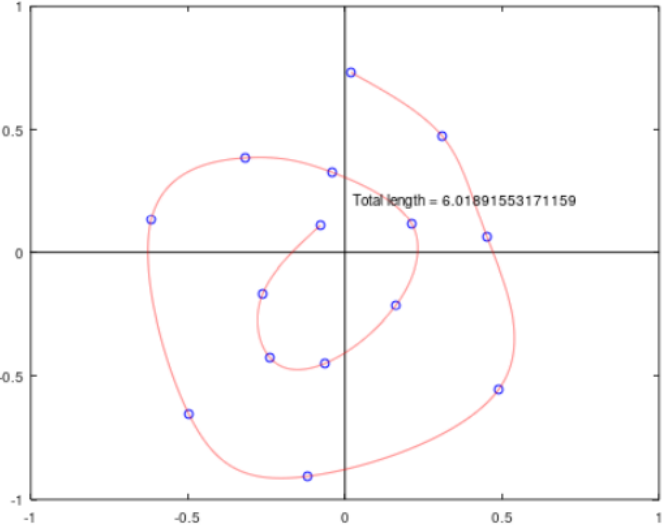
\includegraphics[max size={\textwidth/2}{\textheight}]{soal1-tc1}
	\caption{Contoh Soal \#1: Original}
	\label{fig_tc1}
\end{figure}
Pemanggilan fungsi \emph{parametric spline} menggunakan koordinat yang identik dengan contoh yang telah diberikan pada soal menghasilkan kurva sebagai berikut.
\begin{figure}[H]
	\centering
	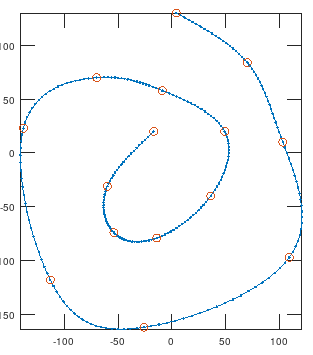
\includegraphics[max size={\textwidth/2}{\textheight}]{anum_tc1_curve}
	\caption{Contoh Soal \#1: Function Output}
	\label{fig_tc1_curve}
\end{figure}
Apabila dibandingkan dengan grafik hasil interpolasi yang diberikan pada soal, dapat dilihat bahwa kurva yang dihasilkan oleh fungsi interpolasi kami memiliki bentuk yang cukup identik dengan grafik asli. Hal ini menunjukkan bahwa algoritma \emph{parametric cubic spline} yang kami gunakan sudah cukup mendekati algoritma yang digunakan untuk membuat contoh pertama pada soal.

Berikut ini merupakan output dari fungsi \(x(t)\) dan \(y(t)\) yang menghasilkan \emph{output} kurva di atas:
\begin{multicols}{2}
	\begin{figure}[H]
		\centering
		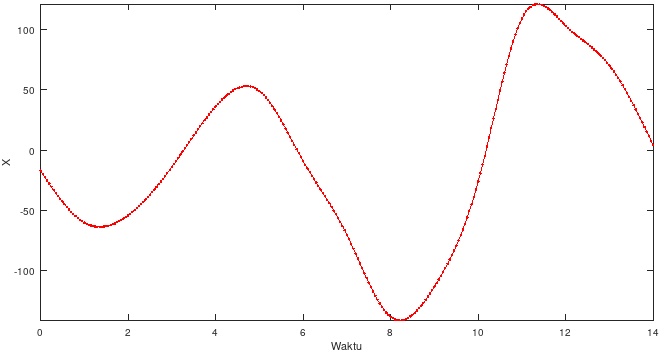
\includegraphics[max size={\textwidth/2}{\textheight}]{anum_tc1_tx.png}
		\caption{Grafik x(t) untuk Kasus I}
		\label{fig_tc1_tx}
	\end{figure}
	\begin{figure}[H]
		\centering
		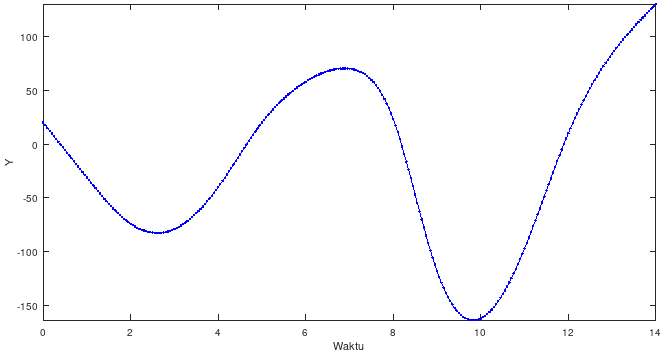
\includegraphics[max size={\textwidth/2}{\textheight}]{anum_tc1_ty.png}
		\caption{Grafik y(t) untuk Kasus I}
		\label{fig_tc1_ty}
	\end{figure}
\end{multicols}
Perhatikan bahwa grafik yang dihasilkan merupakan grafik yang menginterpolasi titik \(t\) terhadap posisi dengan transisi yang cukup halus antara titik-titik pada interval yang sudah diketahui. Menurut kami hasil interpolasi ini sudah cukup memuaskan karena dapat menginterpolasi posisi benda secara baik untuk seluruh interval \(1 \leq t \leq length(position)\) tanpa mengalami diskontinuitas pada hasil interpolasinya.
\subsection{Kasus II: Contoh Soal \#2}
\begin{figure}[H]
	\centering
	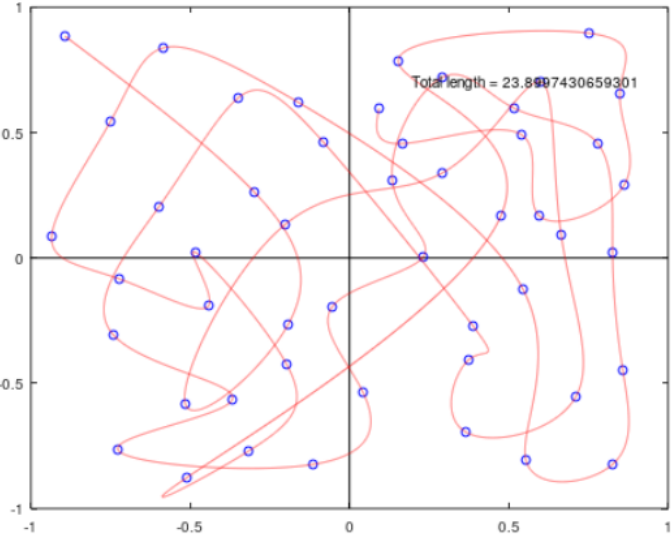
\includegraphics[max size={\textwidth/2}{\textheight}]{soal1-tc2}
	\caption{Contoh Soal \#2: Original}
	\label{fig_tc2}
\end{figure}
Pemanggilan fungsi \emph{parametric spline} menggunakan koordinat yang identik dengan contoh yang telah diberikan pada soal menghasilkan kurva sebagai berikut.
\begin{figure}[H]
	\centering
	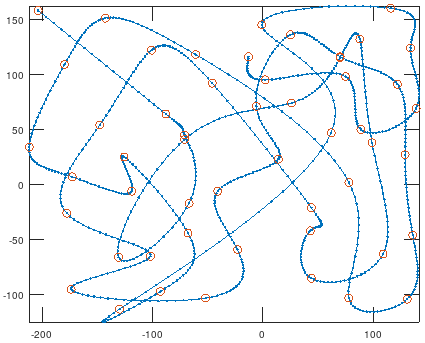
\includegraphics[max size={\textwidth/2}{\textheight}]{anum_tc2_curve}
	\caption{Contoh Soal \#2: Function Output}
	\label{fig_tc2_curve}
\end{figure}
\pagebreak
\begin{multicols}{2}
	\begin{figure}[H]
		\centering
		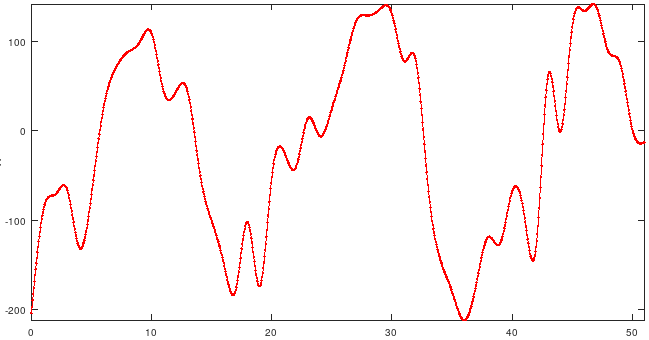
\includegraphics[max size={\textwidth/2}{\textheight}]{anum_tc2_tx.png}
		\caption{Grafik x(t) untuk Kasus II}
		\label{fig_tc2_tx}
	\end{figure}
	\begin{figure}[H]
		\centering
		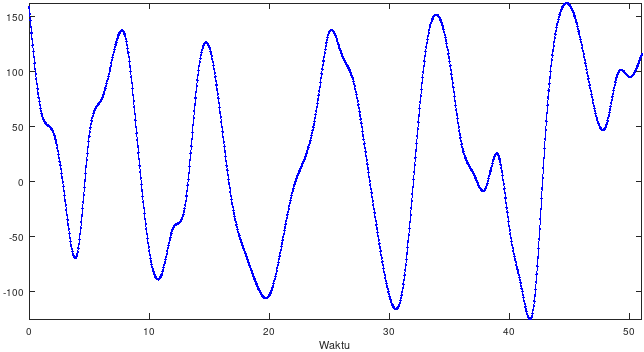
\includegraphics[max size={\textwidth/2}{\textheight}]{anum_tc2_ty.png}
		\caption{Grafik y(t) untuk Kasus II}
		\label{fig_tc2_ty}
	\end{figure}
\end{multicols}
Sama seperti pada bagian sebelumnya, grafik kurva yang dihasilkan oleh fungsi yang telah kami buat memiliki bentuk yang sangat identik dengan contoh yang diberikan pada soal, sehingga kami menyimpulkan bahwa fungsi \emph{parametric spline} yang kami buat sudah memiliki performa yang cukup baik.

\subsection{Kasus III: Amogus}
Selain memiliki manfaat dalam menginterpolasi gerak dari suatu benda yang diketahui posisinya pada detik ke-\(t\), fungsi \emph{parametric spline} yang telah kami bangun dapat juga digunakan untuk melakukan \emph{tracing} pada suatu gambar arbitrer. Pada bagian ini, kami akan melakukan \emph{tracing} pada gambar \emph{meme "Amogus"} untuk mendemonstrasikan potensi aplikasi dari sebuah fungsi \emph{parametric spline}.
\begin{figure}[H]
	\centering
	
\includegraphics[max size={\textwidth/2}{\textheight}]{amogus-original.jpg}
	\caption{Amogus: Original}
\end{figure}

Untuk membuat suatu kurva yang mengaproksimasi bentuk dari gambar tersebut, kami melakukan pemanggilan fungsi dengan koordinat sebagai berikut.
\lstinputlisting{assets/codes/amogus.m}

\begin{figure}[H]
	\centering
	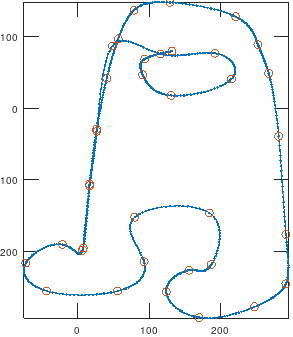
\includegraphics[max size={\textwidth/2}{\textheight}]{amogus_curve.png}
	\caption{Amogus: Function Output}
\end{figure}
Terlihat bahwa fungsi \emph{parametric spline} dapat menghasilkan \emph{outline} gambar yang cukup identik dengan gambar asli yang diberikan di atas. Hal ini mendemonstrasikan salah satu aplikasi dari fungsi \emph{parametric spline} pada bidang \emph{computer graphics} dan \emph{digital art}.

\section{Kompleksitas Algoritma}
\subsection{Kompleksitas Kalkulasi Koefisien}
\lstinputlisting{assets/codes/getSplineCoeff.m}
Asumsikan bahwa \(n\) adalah jumlah pasangan \(x, y\) yang dimasukkan ke fungsi. Perhatikan bahwa pada fungsi yang membuat matriks persamaan, terdapat pemanggilan \emph{floating point operation} sebanyak:
\begin{equation}
	Pengurangan = \sum_{i=2}^{n-1} 8 = 8(n-1) - 8(2) = 8n-24
\end{equation}
\begin{equation}
	Perkalian = \sum_{i=2}^{n-1} 1 = (n-1) - 1(2) = n - 3
\end{equation}
\begin{equation}
	Pembagian = \sum_{i=2}^{n-1} 2 = 2(n-1) - 2(2) = 2n - 6
\end{equation}
Sehingga, dengan asumsi bahwa penyelesaian sistem persamaan akan memakan waktu \(O(n^3)\) (\emph{gaussian elimination}), maka fungsi koefisien akan memiliki kompleksitas sebesar:
\begin{equation}
	Total = O(n^3) + 11n - 33
\end{equation}

Namun, karena matriks permasalahan yang dihasilkan oleh problem ini sudah pasti merupakan matriks \emph{tridiagonal}, dimana elemen non-zero hanya dapat muncul di sebelah diagonal-nya, terdapat algoritma eliminasi yang dapat menyelesaikan persamaan dalam waktu \(O(n)\), yakni algoritma Thomas. Apabila kita asumsikan bahwa penyelesaian permasalahan matriks dilakukan dengan menggunakan algoritma tersebut, maka kompleksitas keseluruhan dari fungsi koefisien akan bernilai:
\begin{equation}
	Total = O(n) + 11n - 33
\end{equation}

\subsection{Kompleksitas Fungsi Interpolant}
\lstinputlisting{assets/codes/naturalSpline.m}
Asumsikan bahwa m adalah jumlah titik yang akan di-interpolasi oleh fungsi \emph{natural spline}. Perhatikan bahwa pada fungsi tersebut, terdapat pemanggilan \emph{floating point operation} sebanyak:
\begin{equation}
	Penjumlahan = \sum_{n=0}^{m} 1 = m
\end{equation}
\begin{equation}
	Pengurangan = \sum_{n=0}^{m} 15 = 15m
\end{equation}
\begin{equation}
	Perkalian = \sum_{n=0}^{m} 5 = 5m
\end{equation}
\begin{equation}
	Pembagian = \sum_{n=0}^{m} 3 = 3m
\end{equation}
Maka, jumlah \emph{floating point opeartion} keseluruhan dari fungsi interpolasi di atas adalah:
\begin{equation}
	Total = Penjumlahan + Pengurangan + Perkalian + Pembagian = 24m
\end{equation}

\subsection{Kompleksitas Fungsi Parametric Spline}
Agar perhitungan \emph{floating point operation} dapat dilakukan dengan lebih mudah, maka fungsi parametric spline yang diberikan di atas kami rubah menjadi bentuk yang lebih sederhana yakni:
\lstinputlisting{assets/codes/simplifiedParametric.m}\
Berdasarkan perhitungan \emph{floating point operation} yang telah dilakukan pada bagian sebelumnya, dan asumsi bahwa \(m = \frac{n}{0.1} = 10n\), maka kompleksitas akhir dari fungsi \emph{paramateric spline} yang telah dibuat adalah:
\begin{equation}
	\begin{split}
		Total & = 2 \times Coefficient + 2 \times Spline\\
		& = O(n^3) + 22n - 66 + 480n\\
		& = O(n^3) + 502n - 66
	\end{split}
\end{equation}


\section{Kesimpulan}
Kesimpulan disini.

% % Example of a table from http://www.latextemplates.com/template/professional-table

\begin{thebibliography}{1}
	% Here are a few examples of different citations 
	% Book
	\bibitem{kopka_1999} % Note the label in the curly brackets. Use the cite the source; e.g., \cite{kopka_latex}
	H.~Kopka and P.~W. Daly, \emph{A Guide to \LaTeX}, 3rd~ed.\hskip 1em plus
	0.5em minus 0.4em\relax Harlow, England: Addison-Wesley, 1999.
	\bibitem{horowitz_2005}D.~Horowitz, \emph{End of Time}. New York, NY, USA: Encounter Books, 2005. [E-book] Available: ebrary, \url{http://site.ebrary.com/lib/sait/Doc?id=10080005}. Accessed on: Oct. 8, 2008.
	% Article from a database
	\bibitem{castlevecchi_2008}D.~Castelvecchi, ``Nanoparticles Conspire with Free Radicals'' \emph{Science News}, vol.174, no. 6, p. 9, September 13, 2008. [Full Text]. Available: Proquest, \url{http://proquest.umi.com/pqdweb?index=52&did=1557231641&SrchMode=1&sid=3&Fmt=3&VInst=PROD&VType=PQD&RQT=309&VName=PQD&TS=1229451226&clientId=533}. Accessed on: Aug.~3, 2014.
	% Conference Paper from the Internet
	\bibitem{lach_2010}J.~Lach, ``SBFS: Steganography based file system,'' in \emph{Proceedings of the 2008 1st International Conference on Information Technology, IT 2008, 19-21 May 2008, Gdansk, Poland.} Available: IEEE Xplore, \url{http://www.ieee.org}. [Accessed: 10 Sept. 2010].
	% Web page, no author
	\bibitem{a_laymans_explanation}``A `layman's' explanation of Ultra Narrow Band technology,'' Oct.~3, 2003. [Online]. Available: \url{http://www.vmsk.org/Layman.pdf}. [Accessed: Dec.~3, 2003].
\end{thebibliography}

% This is a hand-made bibliography. If you want to use a BibTeX file, you're on your own ;-)














\end{document}